% \documentclass[10pt,journal,compsoc]{IEEEtran}
% \usepackage{xeCJK}%preamble part
% \usepackage{graphicx}
% \usepackage{pdfpages}
% \usepackage{indentfirst}
% \usepackage{enumerate}
% \usepackage[a4paper, inner=1.5cm, outer=3cm, top=2cm, bottom=3cm, bindingoffset=1cm]{geometry}
% \usepackage{epstopdf}
% \usepackage{listings}
% \usepackage{array}
% \usepackage{fontspec}
% \usepackage{bm}
% \usepackage{gensymb}
% \usepackage{todonotes}
% \usepackage{amsmath, amsthm, amssymb}
% \usepackage[citecolor=blue]{hyperref}
% \newtheorem{definition}{Definition}
%\newtheorem{thm}{Theorem}[section]
% \newtheorem{thm}{Theorem}
% \newtheorem{corollary}{Corollary}
% \newtheorem{lem}{Lemma}
% \newtheorem{remark}{Remark}
% \newtheorem{proposition}{Proposition}
% \DeclareMathOperator{\sgn}{sgn}
% \theoremstyle{remark}
% \newtheorem*{rem}{Remark}
% \setCJKmainfont[BoldFont={SimHei}]{SimSun}
% \setCJKmonofont{SimSun}
% \setmainfont{Times New Roman}
% \newCJKfontfamily[hei]\heiti{SimHei}
% \setlength{\extrarowheight}{4pt}
% \setlength{\parindent}{1cm}
 
%\begin{document}
\title{第二篇--协作定位网络中的时空信息耦合$^{[2]}$} 
%\author{\fontsize{12pt}{\baselineskip}{沈渊,清华大学电子工程系副教授}}
%\markboth{Journal of \LaTeX\ Class Files,~Vol.~14, No.~8, August~2015}%
%{Shell \MakeLowercase{\textit{et al.}}: Bare Advanced Demo of IEEEtran.cls for IEEE Computer Society Journals}
%\IEEEtitleabstractindextext{
%\begin{abstract}
\textbf{摘要}:%第二篇论文翻译,原文的题目是
%Spatio-Temporal Information Coupling in Cooperative Network Navigation
%原文的摘要翻译如下:
可靠的定位信息对很多基于位置的应用起着至关重要的作用。通过时空联合协作的网络导航可以给移动节点提供高精度和鲁棒的位置信息。同时,由于待测节点的位置相关,这种联合协作导致了错综复杂的信息获取方式,也就是信息耦合的问题。在这篇文章中,通过对费舍尔信息量的分析,我们在四种有代表性的情形中量化了信息耦合。我们说明了每个节点所获得的信息来自与它进行时空协作的节点和由于和邻居节点的协作产生的信息耦合。我们的结果为网络中复杂信息获取提供了洞见,并且能够为高效的网络导航算法提供指导。
%\end{abstract}
%}\maketitle
%reset section counter here
\setcounter{section}{0}
\section{简介}
关于研究背景的翻译略去,下面是原文一些记号上的约定。
$[\cdot]^T$表示变量的转置;$\mathbb{S}^D,\mathbb{S}^D_+,\mathbb{S}^D_{++}$分别表示$D\times D$的实矩阵、半正定矩阵和正定矩阵。$\bm{J}_r(\bm{v}):=\bm{v}\bm{v}^T$表示由向量$\bm{v}$做外积得到的秩1阵。
另外$\angle \{ \bm{u},\bm{v}\}
$表示向量$\bm{u}$和向量$\bm{v}$之间的夹角。
\section{网络导航中的费舍尔信息量}
在本节中,我们首先介绍网络模型和网络导航中的FIM作为预备知识,然后描述这篇文章重点讨论的4种场景。
\subsection{预备知识}
考虑一个由若干节点构成的协作网络,用$\bm{x}_k^{(n)}\in \mathbb{R}^D$表示节点k在时间$t_n$的位置状态,$k=1,2,....,N$且$n=1,2,...T$.网络导航的目标是从测量和先验信息中推断节点的位置信息。
令$\mathcal{S}=\{1,2,...,S\}\text{ with }S=N\cdot T$是位置状态的下标集,文献[8]已经证明了对于S个位置状态FIM可以分解成:
\begin{equation}
\bm{J}=\sum_{(i,j)\in \mathcal{S}^2,i\geq j} \bm{G}^S_{i,j} \otimes \bm{K}_{i,j}
\end{equation}
其中$\otimes$表示Kronecker矩阵积,$S\times S$的矩阵$\bm{G}^S_{i,j}$的元素$(k,r)$由下式给出:
\[
[\bm{G}^S_{i,j}]_{k,r}=\left\{
\begin{array}{c l}	
     1 & k=r=i\\
     1 & k=r=j\\
     -1 & k=i,r=j,k \neq r\\
     -1 & k=j,r=i,k \neq r\\
     0, & \text{otherwise}
\end{array}\right.
\]
$\bm{K}_{i,j}\in \mathbb{S}_+^D$ 描述了包含在测量或先验知识中和位置状态i,j有关的位置信息。$\bm{K}_{i,j}=\bm{K}_{j,i}$并且在缺少关于位置状态i,j的测量或先验知识的情况下$\bm{K}_{i,j}=0$。特别的,如果$i=j$,$\bm{K}_{i,i}$描述了仅仅和位置状态i有关的位置信息。
\subsection{有代表性的场景}
我们考虑图1中的四种场景以获得对时空协作的洞见。
\begin{figure}
\centering
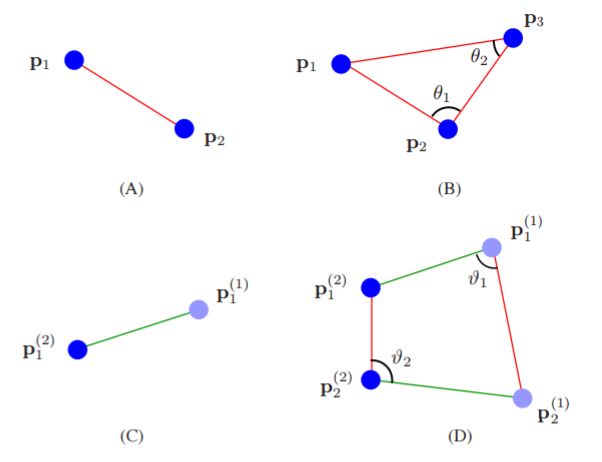
\includegraphics[width=\textwidth/2]{figure_1.png}
\caption{四种场景:(A)两个节点的空间协作(红色的连接);(B)三个节点的空间协作;(C)一个节点的时间协作(绿色的连接);(D)两个节点的时空协作。}
\end{figure}

在这些场景中,位置状态就是节点的位置,节点通过和位置已知的锚点和位置未知的邻居节点的测距中获得位置信息。
在接下来的讨论中,在时间步为n时,$\bm{K}^{(n)}_{i,i}$表示节点i从锚点获取的信息;$\bm{u}_{i,j}^{(n)}$表示节点i和j连线的单位方向向量;$\lambda^{(n)}_{i,j}=\lambda^{(n)}_{j,i}$表示节点i和j之间的测距信息强度(RII);$\bm{u}_{i,i}^{(n)}$表示链接节点i在时间步为n和n+1时的位置的单位方向向量;$\lambda^{(n)}_{i,i}$表示节点i的速度信息强度(SII)。

\textbf{场景A:}两个节点通过彼此测距协作来确定它们的位置,即位置状态是$\bm{p}_1$和$\bm{p}_2$,测距信息是$\bm{J}_r(\bm{v}_{1,2})$,其中$\bm{v}_{1,2}=\sqrt{\lambda_{1,2}}\bm{u}_{1,2}$,因此,基于(1)式我们得到这种场景的FIM是:
\begin{equation}
\bm{J}_A=\left[
\begin{array}{cc}
\bm{K}_{1,1}+\bm{J}_r(\bm{v}_{1,2})&-\bm{J}_r(\bm{v}_{1,2})\\
-\bm{J}_r(\bm{v}_{1,2})&\bm{K}_{2,2}+\bm{J}_r(\bm{v}_{1,2})\\
\end{array}
\right]
\end{equation}
%\begin{figure*}[!t]
\begin{equation*}
\bm{J}_B=\left[
\begin{array}{ccc}
\bm{K}_{1,1}+\bm{J}_r(\bm{v}_{1,2})+\bm{J}_r(\bm{v}_{1,2}) & -\bm{J}_r(\bm{v}_{1,2}) & -\bm{J}_r(\bm{v}_{1,3})\\
-\bm{J}_r(\bm{v}_{1,2}) &\bm{K}_{2,2}+\bm{J}_r(\bm{v}_{1,2})+\bm{J}_r(\bm{v}_{2,3}) & -\bm{J}_r(\bm{v}_{2,3})\\
 -\bm{J}_r(\bm{v}_{1,3}) & -\bm{J}_r(\bm{v}_{2,3})&
\bm{K}_{3,3}+\bm{J}_r(\bm{v}_{1,3})+\bm{J}_r(\bm{v}_{2,3})\\
\end{array}
\right]
\end{equation*}
%\hrulefill
%\vspace*{4pt}
%\end{figure*}

\textbf{场景B:} 三个节点通过彼此测距协作确定它们的位置,即位置状态是$\bm{p}_1,\bm{p}_2$和$\bm{p}_3$,测距信息是$\bm{J}_r(\bm{v}_{i,j})$对于$i,j\in \{1,2,3\},i\neq j$,其中$\bm{v}_{i,j}=\sqrt{\lambda_{i,j}}\bm{u}_{i,j}$,因此,基于式(1)我们可以得到这种情形的FIM由(3)给出,在下一页的最开始的地方。

\textbf{场景C:}单节点在两个不同的时刻通过速度测量协作来确定自身的位置,即位置状态是$\bm{p}^{(1)}_1$和$\bm{p}^{(2)}_1$,速度测量的信息是$\bm{J}_r(\bm{t})$,其中$\bm{t}=\sqrt{\lambda^{(1)}_{1,1}}\bm{u}_{1,1}^{(1)}$.因此基于(1),我们得到这种场景的FIM是:
\[\bm{J}_C=\left[
\begin{array}{cc}
\bm{K}_{1,1}^{(1)}+\bm{J}_r(\bm{t})&-\bm{J}_r(\bm{t})\\
-\bm{J}_r(\bm{t})&\bm{K}_{2,2}^{(2)}+\bm{J}_r(\bm{t})\\
\end{array}\right]
\]

\textbf{场景D:}两个节点在两个不同的时刻协作来确定它们的位置,即,位置状态是$\bm{p}_1^{(1)},\bm{p}_2^{(1)},\bm{p}_1^{(2)}$和$\bm{p}_2^{(2)}$,每个节点测量自身的速度和相对另一节点的距离,并且
\begin{itemize}  
\item 测距信息是$\bm{J}_r(\bm{v}_{1,2})$和$\bm{J}_r(\bm{w}_{i,j})$,其中$\bm{v}_{1,2}=\sqrt{\lambda_{1,2}^{(1)}}\bm{u}^{(2)}_{1,2}$,而$\bm{w}_{1,2}=\sqrt{\lambda_{1,2}^{(2)}}\bm{u}^{(1)}_{1,2}$
\item 测速信息是$\bm{J}_r(\bm{t}_1)$和$\bm{J}_r(\bm{t}_2)$,其中$\bm{t}_i=\sqrt{\lambda_{i,i}^{(1)}}\bm{u}^{(1)}_{i,i}$
\end{itemize}
因此,基于(1)式我们得到这种类形的FIM是
\[
\bm{J}_D=\left[
\begin{array}{cc}
\bm{J}^{(1)}_A+\bm{T}&-\bm{T}\\
-\bm{T}&\bm{J}^{(2)}_A+\bm{T}\\
\end{array}
\right]
\]
其中$\bm{J}^{(1)}_A$和$\bm{J}^{(2)}_A$由(2)式给出,上标代表了时间步长,$\bm{T}=\text{diag}\{\bm{J}_r(\bm{t}_1),\bm{J}_r(\bm{t}_2)\}$.
\section{空间信息耦合}
在这一节中,我们推导了场景A和场景B的EFIM,并且描述了场景B中由于空间协作导致的信息耦合。由于篇幅所限,这篇文章的大部分证明略去。
\begin{proposition}
场景A中节点1的EFI是
\[
\bm{J}_e=\bm{K}_{1,1}+(1-\mu_2^{1,1})\bm{J}_r(\bm{v}_{1,2})
\]
其中
\begin{eqnarray*}
\mu_2^{1,1}=&\bm{v}^T_{1,2}(\bm{K}_{2,2}+\bm{J}_r(\bm{v}_{1,2}))^{-1}\bm{v}_{1,2}\\
=&1-(1+\lambda_{1,2}\bm{u}^T_{1,2}\bm{K}^{-1}_{2,2}\bm{u}_{1,2})^{-1}.
\end{eqnarray*}
此外,$\bm{J}_e \preceq \bm{K}_{1,1}+\bm{J}_r(\bm{v}_{1,2}).$
\end{proposition}
\begin{remark}
场景A中节点1的EFIM是来自锚点和来自与节点2的协作的信息之和。协作在与节点2的连线方向上增加了信息,而节点1可以有效利用的RII随RII $\lambda_{1,2}$增大而增大而随节点2位置在$\bm{u}_{1,2}$方向的不确定性(即$\bm{u}^T\bm{K}^{-1}_{2,2}\bm{u}_{1,2}$)的增大而减小。此外,有效RII总是小于或等于RII。当锚点在节点1,2连线方向上给节点2提供无穷大的信息量时取等号,而当锚点
在这一方向上不提供任何信息时取0。
\end{remark}
\begin{proposition}
在场景B中节点1的EFIM是
\begin{equation}
\begin{split}
\bm{J}_e=\bm{K}_{1,1}+(1-\mu_2^{1,1})\bm{J}_r(\bm{v}_{1,2})+(1-\mu_3^{1,1})\bm{J}_r(\bm{v}_{1,3})\\
+\delta\bm{J}_r(\mu_2^{1,3}\bm{v}_{1,2}+\mu_3^{1,2}\bm{v}_{1,3})
\end{split}
\end{equation}
其中$\mu_i^{j,k}=\bm{v}^T_{j,i}(\bm{K}_{i,i}+\bm{J}_r(\bm{v}_{1,i}))^{-1}\bm{v}_{k,i}$,并且$\delta=(1+\mu_2^{3,3}+\mu_3^{2,2})^{-1}$.除此之外,$\bm{J}_e \preceq \bm{K}_{1,1}+\bm{J}_r(\bm{v}_{1,2})+\bm{J}_r(\bm{v}_{1,3})$.
\end{proposition}
\begin{remark}
命题2说明了场景B下节点1的EFIM是4项的和。第一项对应着从锚点获取的信息,其他三项对应着由于空间协作获得的信息。第二项和第三项对应着沿着与节点2和节点3的连线方向获取的有效信息,而最后一项代表着由于节点2和3协作造成的信息耦合。最后一项是一个秩一阵,有一个非负的特征值$\delta ||\mu_2^{1,3}\bm{v}_{1,2}+\mu_3^{1,2}\bm{v}_{1,3}||^2$并且这个特征值对应的特征向量是$\mu_2^{1,3}\bm{v}_{1,2}+\mu_3^{1,2}\bm{v}_{1,3}$,这个方向既依赖于RII,又依赖于节点2和3位置的不确定性,还和节点的空间拓扑有关。
\end{remark}
接下来我们将说明节点2和3的协作强度如何影响节点1的EFIM.
\begin{corollary}
设$\lambda_{2,3}$和$\tilde{\lambda}_{2,3}$分别表示节点2和节点3之间两个RII,并且$(\mu_2^{1,3},\mu_3^{1,2},\delta),(\tilde{\mu}_2^{1,3},\tilde{\mu}_3^{1,2},\tilde{\delta})$分别表示命题2中对应的两组参数,而其他参数均相同。那么:
\begin{equation}
\delta \bm{J}_r(\mu_2^{1,3}\bm{v}_{1,2}+\mu_3^{1,2}\bm{v}_{1,3}) \preceq \tilde{\delta} \bm{J}_r(\tilde{\mu}_2^{1,3}\bm{v}_{1,2}+\tilde{\mu}_3^{1,2}\bm{v}_{1,3})
\end{equation}
当且仅当$\lambda_{2,3}\leq \tilde{\lambda}_{2,3}$。此外
\[
\lim_{\lambda_{2,3} \rightarrow \infty}\delta \bm{J}_r(\mu_2^{1,3}\bm{v}_{1,2}+\mu_3^{1,2}\bm{v}_{1,3})=\bar{\delta} \bm{J}_r(\bar{\mu}_2^{1,3}\bm{v}_{1,2}+\bar{\mu}_3^{1,2}\bm{v}_{1,3})
\]
其中
\[
\bar{\mu}_2^{1,3}=\bm{v}_{1,2}^T(\bm{K}_{2,2}+\bm{J}_r(\bm{v}_{1,2}))^{-1}\bm{u}_{2,3}
\]
\[
\bar{\mu}_3^{1,2}=\bm{v}_{1,3}^T(\bm{K}_{3,3}+\bm{J}_r(\bm{v}_{1,3}))^{-1}\bm{u}_{2,3}
\]
\[
\bar{\delta}=(\bm{u}_{2,3}^T((\bm{K}_{2,2}+\bm{J}_r(\bm{v}_{1,2}))^{-1}+(\bm{K}_{3,3}+\bm{J}_r(\bm{v}_{1,3}))^{-1})\bm{u}_{2,3})^{-1}.
\]
\end{corollary}
\begin{remark}
从(5)中可以知道,当节点2,3方向保持不变时,节点1从和节点2和3协作中获得的信息随着节点2和3之间的RII的增大而增大。另外,这个信息量的上界是在节点2和3之间测距是理想情况时取得。
\end{remark}
在下面这个推论中,我们将说明如果从协作中获得的信息是分别和节点2,节点3的测距信息的加权和这种情形。
\begin{corollary}
场景B中节点1的EFIM可以写成
\[
\bm{J}_e=\bm{K}_{1,1}+\eta_1 \bm{J}_r(\bm{v}_{1,2})+\eta_2 \bm{J}_r(\bm{v}_{1,3}),\eta_1,\eta_2 \geq 0
\]
当且仅当至少下面至少有一个条件满足:
\begin{itemize}
\item{三个节点共线}
\item $\lambda_{1,2}\cdot \lambda_{1,3}\cdot \lambda_{2,3}=0$
\item $\bm{u}_{1,2}^T(\bm{K}_{2,2}+\bm{J}_r(\bm(v)_{1,2}))^{-1}\bm{u}_{2,3}=0$
\item $\bm{u}_{1,3}^T(\bm{K}_{3,3}+\bm{J}_r(\bm(v)_{1,3}))^{-1}\bm{u}_{2,3}=0$
\end{itemize}
\end{corollary}
接下来我们将说明如果锚点提供各向同性的信息给节点2,3,那么权重参数$\mu_i^{j,k}$可以写成$\theta_1=\angle \{\bm{u}_{1,2},\bm{u}_{2,3}\}$和$\theta_2=\angle \{\bm{u}_{1,3},\bm{u}_{2,3}\}$的函数。
\begin{corollary}
如果$\bm{K}_{i,i}=\xi_i\bm{I}$对于$i=2,3$成立,则场景B中节点1的EFIM为
\begin{equation*}
\begin{split}
\bm{J}_e=\bm{K}_{1,1}+\frac{\xi_2}{\xi_2+\lambda_{1,2}}\bm{J}_r(\bm{v}_{1,2})+\frac{\xi_3}{\xi_3+\lambda_{1,3}}\bm{J}_r(\bm{v}_{1,3})\\
+\delta\bm{J}_r(\mu_2^{1,3}\bm{v}_{1,2}+\mu_3^{1,2}\bm{v}_{1,3})
\end{split}
\end{equation*}
其中
\[
\mu_2^{1,3}=\frac{\sqrt{\lambda_{1,2}\lambda_{2,3}}\cos \theta_1}{\xi_2+\lambda_{1,2}}
\]
\[
\mu_3^{1,2}=\frac{\sqrt{\lambda_{1,3}\lambda_{2,3}}\cos \theta_2}{\xi_3+\lambda_{1,3}}
\]
\[
\mu_2^{3,3}=\frac{\lambda_{2,3}}{\xi_2}(1-\frac{\lambda_{1,2}\cos^2 (\theta_2)}{\xi_2+\lambda_{1,2}})
\]
\[
\mu_3^{2,2}=\frac{\lambda_{2,3}}{\xi_3}(1-\frac{\lambda_{1,3}\cos^2 (\theta_2)}{\xi_3+\lambda_{1,3}})
\]
\end{corollary}
\begin{remark}
这个结果说明了如果$(i)$节点2和3来自锚点或先验的信息是各向同性的$(ii)\bm{u}_{1,2}\perp\bm{u}_{2,3}$或者$\bm{u}_{1,3}\perp\bm{u}_{2,3}$,那么节点1通过写作获得的信息是分别来自节点2的测距信息的加权和。
\end{remark}
\section{空时信息耦合}
在本节中,我们推导出了场景C和D下节点1在时间步2时的EFIM,并且描述了场景D中由于空时协作产生的信息耦合。
\begin{proposition}
场景C中节点1的EFIM是
\[
\bm{J}_e=\bm{K}_{1,1}^{(2)}+\frac{\lambda_{1,1}^{(1)}}{1+\lambda_{1,1}^{(1)}\bm{u}_{1,1}^T(\bm{K}_{1,1}^{1})^{-1}\bm{u}_{1,1}}\bm{J}_r(\bm{u}_{1,1})
\]
此外$\bm{J}_e \preceq \bm{K}_{1,1}^{(2)}+\bm{J}_r(\bm{t})$.
\end{proposition}
\begin{remark}
与场景A类似,场景C中时间步为2时节点1的EFIM是从锚点获取的信息和与节点1在时间步为1时的协作信息之和。协作在节点1在两个时刻位置连线的方向上增加了信息,而节点1可以有效利用的SII随SII $\lambda_{1,1}^{(1)}$的增加而增大而随着节点1在时间步1的位置不确定性(即方向$\bm{u}_{1,1}^T(\bm{K}_{1,1}^{(1)})^{-1}\bm{u}_{1,1}$)的增大而减小。此外,有效的SII总是小于等于SII,当锚点给时间步1时的节点提供无穷大的信息时取等号,当不提供任何信息时取0.
\end{remark}
\begin{proposition}
场景D中节点1在时间步2时的EFIM是
\begin{equation}
\begin{split}
\bm{J}_e=\bm{K}_{1,1}^{(2)}+&[1-\bm{v}_{1,2}^T(\bm{K}_{2,2}^{(2)}+\bm{H}_{1,2})^{-1}\bm{v}_{1,2}]\bm{J}_r(\bm{v}_{1,2})\\
+&[1-\bm{t}_1^T(\bm{K}_{1,1}^{(1)}+\bm{H}_{1,1})^{-1}\bm{t}_1]\bm{J}_r(\bm{t}_1)\\
+&\delta \bm{J}_r(\nu_2 \bm{v}_{1,2}+\nu_1 \bm{t}_1)
\end{split}
\end{equation}
此外$\bm{J}_e \preceq \bm{K}_{1,1}^{(2)}+\bm{J}_r(\bm{v}_{1,2})+\bm{J}_r(\bm{t}_1)$
\end{proposition}
\begin{remark}
和场景B类似,命题4说明了在场景D中,时间步2时节点1的EFIM是4项的和。第一项对应着从锚点获得的信息,其余的项对应着通过协作获得的信息。第二和第三项分别是节点2在时间步2和节点1进行空间协作以及和自身在时间步1的时间协作获得的信息。而最后一项对应着耦合项。最后一项是一个秩一阵,有一个非负的特征值为$\delta||\nu_2\bm{v}_{1,2}+\nu_1\bm{t}_1||^2$,对应的特征向量为$\nu_2\bm{v}_{1,2}+\nu_1\bm{t}_1$。这个方向依赖于RII,SII,协作节点位置的不确定度以及节点在空间上的拓扑。特别的,当$\bm{t}_2^T(\bm{K}_{2,2}^{(1)})^{-1}\bm{w}_{1,2}=0$时,比如$\bm{K}_{2,2}^{(1)}=\xi_{2,2}^{(1)}\bm{I}$且$\bm{u}_{1,2}^{(1)} \perp\bm{u}_{2,2}^{(1)}$,最后一项为0.
\end{remark}
\section{数值结果}
在本节中,我们给出若干个含有信息耦合的EFIM的数值的例子。特别的,我们将考察节点的网络拓扑如何影响信息耦合项。

信息耦合项是协作节点方向加权组合作外积得到的,对于场景B,权系数是$\sqrt{\delta}\mu_2^{1,3}$和
$\sqrt{\delta}\mu_3^{1,2}$,对于场景D权系数是$\sqrt{\delta}\nu_2$和
$\sqrt{\delta}\nu_1$,图2和图3分别说明了这些系数对于角度$\theta_1=\angle \{\bm{u}_{1,2},\bm{u}_{2,3}\},\theta_2=\angle \{\bm{u}_{1,3},\bm{u}_{2,3}\}$或者$\vartheta_1=\angle \{\bm{u}_{1,1},\bm{u}_{1,2}^{(1)}\},\vartheta_2=\angle \{\bm{u}_{2,2},\bm{u}_{1,2}^{(2)}\}$的依赖关系。在数值结果里,我们设
$\bm{K}_{2,2}=\bm{K}_{3,3}=\bm{K}_{2,2}^{(2)}=\bm{K}_{2,2}^{(1)}=\bm{K}_{1,1}^{(1)}=\bm{I}$,所以的RII和SII都取1,并且$\bm{u}_{1,1}^T\bm{u}_{1,2}^{(2)}=0$.

在图2中,我们可以看到$\sqrt{\delta}\mu_2^{1,3}$和$\sqrt{\delta}\mu_3^{1,2}$,即$\bm{v}_{1,2}$或$\bm{v}_{1,3}$的权重,当$\bm{u}_{1,2}$和$\bm{u}_{1,3}$正交于$\bm{u}_{2,3}$时分别为0.此外,这两项在节点1,2,3共线时达到最大值。

类似的,在图3中,我们可以看到$\sqrt{\delta}\nu_2$和$\sqrt{\delta}\nu_1$,即耦合项中$\bm{v}_{1,2}$或$\bm{t}_1$的系数,当$\bm{u}_{2,2}$正交于$\bm{u}_{1,2}^{(2)}$且$\bm{u}_{1,1}$正交于$\bm{u}_{1,2}^{(1)}$时分别为0。此外,这两项当节点2在时间步1和2与节点1在时间步2共线或者节点1在时间步1和2与节点2在时间步1共线时为0.
%\section{结论}
%略
%\begin{thebibliography}{1}
%\item{略}
%\end{thebibliography}
%证明思路,找到一个数,对这个数求逆
%\includepdf{page5.pdf}
%\end{document}